%% Diambil dari buku Data and Computer Communications, 8th Edition
\chapter{Data Link Control Protocol}

\section{Key Points}
\begin{itemize}
	\item Karena kemungkinan kesalahan transmisi, dan karena penerima data (\textit{receiver}) mungkin perlu mengatur kecepatan kedatangan data (\textit{data rate}), maka tidak cukup hanya dengan teknik sinkronisasi dan antarmuka (\textit{interface}). Perlu untuk menerapkan lapisan kontrol (\textit{layer of control}) di setiap perangkat komunikasi yang menyediakan fungsi seperti kontrol aliran (\textit{flow control}), deteksi kesalahan (\textit{error detection}), dan kontrol kesalahan (\textit{error control}). Lapisan kontrol (\textit{layer of control}) ini dikenal sebagai \textit{data link control protocol}.

	\item \textit{Flow control} memungkinkan penerima (\textit{receiver}) untuk mengatur aliran data dari pengirim sehingga \textit{buffer} penerima tidak meluap (\textit{overflow}).
	
	\item Dalam \textit{data link control protocol}, \textit{error control} dicapai dengan transmisi ulang \textit{frame} rusak yang belum diakui atau yang meminta transmisi ulang oleh pihak lain.
	
	\item \textit{High-level data link control} (HDLC) adalah \textit{data link control protocol} yang banyak digunakan. Ini berisi hampir semua fitur yang ditemukan di \textit{data link control protocol} lainnya.
\end{itemize}


\section{Pengantar}

Diskusi kita sejauh ini berkaitan dengan pengiriman sinyal melalui tautan transmisi (\textit{transission link}). Untuk komunikasi data digital yang efektif, lebih banyak yang dibutuhkan untuk mengontrol dan mengelola pertukaran data. Dalam bab ini, kami mengalihkan penekanan kami ke pengiriman data melalui tautan komunikasi data (\textit{data communication link}). Untuk mencapai kontrol yang diperlukan, lapisan logika (\textit{layer of logic}) ditambahkan di atas \textit{physical layer} yang dibahas dalam Bab \ref{ch:06}; logika ini disebut sebagai \textit{data link control} atau \textit{data link control protocol}. Ketika \textit{data link control protocol} digunakan, media transmisi antar sistem disebut sebagai \textit{data link}.

Untuk melihat kebutuhan terhadapt \textit{data link control}, kami membuat daftar beberapa persyaratan dan tujuan untuk komunikasi data yang efektif antara dua stasiun pemancar dan penerima yang terhubung langsung:

\begin{itemize}
	
	\item \textit{Frame synchronization}: Data dikirim dalam blok yang disebut \textit{frame}. Bagian awal dan akhir setiap \textit{frame} harus dapat dikenali. Kami secara singkat memperkenalkan topik ini dengan diskusi tentang \textit{synchronous frames} (Gambar \ref{fig:06.02}).

	\item \textit{Flow control}: Stasiun pengirim tidak boleh mengirim \textit{frame} dengan kecepatan yang lebih cepat daripada yang dapat diserap oleh stasiun penerima.
	
	\item \textit{Error control}: \textit{Bit error} yang diperkenalkan oleh sistem transmisi harus diperbaiki.
	
	\item \textit{Addressing}: Pada sebuah \textit{shared link}, seperti \textit{local area network} (LAN), identitas dari dua stasiun yang terlibat dalam transmisi harus ditentukan.
	
	\item \textit{Control} dan data pada \textit{link} yang sama: Biasanya tidak diinginkan untuk memiliki jalur komunikasi yang terpisah secara fisik untuk \textit{control information}. Oleh karena itu, penerima harus dapat membedakan \textit{control information} dari data yang dikirim.
	
	\item \textit{Link management}: Inisiasi, pemeliharaan, dan penghentian pertukaran data yang berkelanjutan membutuhkan koordinasi dan kerja sama yang cukup di antara stasiun. Prosedur untuk pengelolaan pertukaran ini diperlukan.
\end{itemize}

Tak satu pun dari persyaratan ini dipenuhi oleh teknik yang dijelaskan dalam Bab \ref{ch:06}. Kita akan melihat dalam bab ini bahwa \textit{data link protocol} yang memenuhi persyaratan ini adalah hal yang agak rumit. Kami mulai dengan melihat dua mekanisme utama yang merupakan bagian dari \textit{data link control}: \textit{flow control} dan \textit{error control}. Mengikuti latar belakang ini, kami melihat contoh terpenting dari \textit{data link control protocol}: HDLC (\textit{high-level data link control}). Protokol ini penting karena dua alasan: Pertama, ini adalah standar \textit{data link control protocol} yang banyak digunakan. Kedua, HDLC berfungsi sebagai \textit{baseline} yang mana hampir semua \textit{data link control protocol} penting lainnya diturunkan. Akhirnya, lampiran bab ini membahas beberapa masalah kinerja yang berkaitan dengan \textit{data link control}.


\section{Flow Control}

\textit{Flow control} adalah teknik untuk memastikan bahwa entitas pengirim tidak membanjiri entitas penerima dengan data. Entitas penerima biasanya mengalokasikan \textit{buffer data} dengan beberapa panjang maksimum untuk transfer. Saat data diterima, penerima harus melakukan sejumlah pemrosesan sebelum meneruskan data ke \textit{software} tingkat yang lebih tinggi. Jika tidak ada \textit{flow control}, \textit{buffer} penerima mungkin terisi dan meluap saat memproses data lama.

Untuk memulai, kami memeriksa mekanisme \textit{flow control} jika tidak ada \textit{error}. Model yang akan kita gunakan digambarkan pada Gambar \ref{fig:07.01}a, yang merupakan diagram urutan waktu vertikal. Ini memiliki keuntungan dalam menunjukkan ketergantungan waktu dan menggambarkan hubungan kirim-terima yang benar. Setiap panah mewakili satu frame yang menghubungkan tautan data antara dua stasiun. Data dikirim dalam urutan bingkai, dengan setiap bingkai berisi sebagian data dan beberapa informasi kontrol. Waktu yang dibutuhkan stasiun untuk memancarkan semua bit frame ke medium adalah waktu transmisi; ini sebanding dengan panjang frame. Waktu propagasi adalah waktu yang dibutuhkan sedikit untuk melintasi tautan antara sumber dan tujuan. Untuk bagian ini, kami berasumsi bahwa semua frame yang dikirimkan berhasil diterima; tidak ada bingkai yang hilang dan tidak ada yang datang dengan kesalahan. Selain itu, bingkai tiba dalam urutan yang sama seperti saat dikirim. Namun, setiap frame yang ditransmisikan mengalami jumlah penundaan yang berubah-ubah dan variabel sebelum penerimaan.\footnotemark

\footnotetext{ 
	On a direct point-to-point link, the amount of delay is fixed rather than variable. However, a data link control protocol can be used over a network connection, such as a circuit-switched or ATM network, in which case the delay may be variable.
}

\begin{figure}
	\centering
	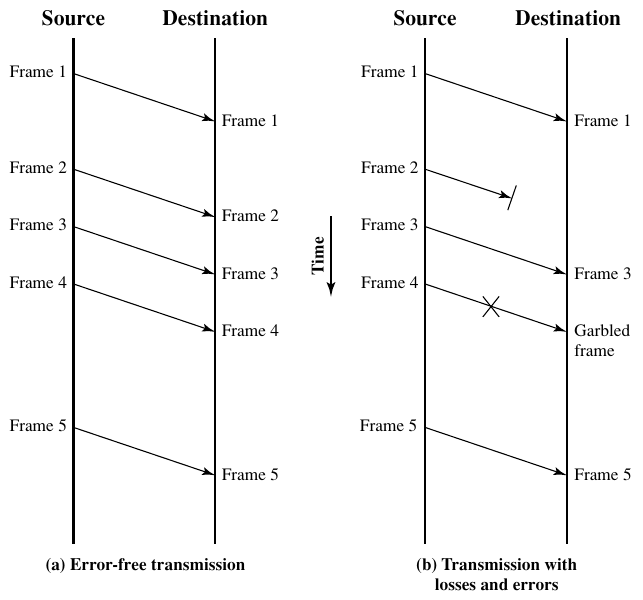
\includegraphics[width=0.7\linewidth]{gambar/fig:07.01}
	\caption{Model dari Frame Transmission}
	\label{fig:07.01}
\end{figure}

\subsection{Stop-and-Wait Flow Control}

\textit{Flow control} yang paling sederhana adalah \textbf{stop-and-wait flow control}. Cara kerja dari flow control ini adalah sebagai berikut. Sebuah sumber akan mentransmisikan sebuah \textit{frame}.

\section{Error Control}


\section{High-Level Data Link Control (HDLC)}
